\section{Neural Networks as Function Approximators}
\label{ch1:sec3}

In this section we introduce artificial neural networks, usually just called neural networks, which are computing systems inspired by the biological neural networks that constitute animal brains. They can be used to model complex relationships between inputs and outputs or to find patterns in data. It has been shown that these systems can be used very well as classifiers as well as regressors or function approximators. \\
Artificial neural networks are based on simplified models of biological neurons, which are special cells within the nervous system which transmit information to other nerve cells. Each of these artificial neurons receives an input value, e.g. a real-valued vector, modifies it with weights and forms a biased sum. Subsequently, an activation function controls the amplitude of the output. These artificial neurons, or just neurons, are connected to each other. A single neuron may be connected to many other neurons and the total number of neurons and connections in a network may be extensive. The connections of the biological neuron are modelled as weights. Each weight determines one neuron's influence on another, a positive weight reflects an excitatory connection, while a negative weight means an inhibitory connection. The other neurons connected to this neuron take the output of this neuron as part of their input and modify it with the weight of the corresponding connection. Then the whole process is repeated. \\
However, artificial neural networks are more about an abstraction of that information processing, less about replicating biological neural networks and neurons. In 1958, the psychologist Frank Rosenblatt invented the first mathematical model for a single neuron, termed perceptron, in \cite{Rosenblatt:1958}, which was also the first artificial neural network. We want to use artificial neurons based on the perceptron and the neural networks constructed from them to approximate the function values of the solution of the differential equation.  \\
Let us We describe how a single artificial neuron transforms a reel-valued input into a one-dimensional output, as illustrated in \cref{fig4}. Let there be $n$ input values $x_1, \ldots, x_n \in \mathbb{R}$, which can be understood as the entries of a vector $x \in \mathbb{R}^n$. First one forms a biased linear combination with the input values, i.e. 
\begin{equation*}
    a = \sum^{n}_{i=1} w_i x_i + b = w^{\mathrm{T}} x + b,
\end{equation*}
where $w_1, \ldots, w_n \in \mathbb{R}$ are called weights and $b \in \mathbb{R}$ is called bias. In general, these weights and the bias are learned through data, which will be provided by the user. The weighted sum $a$ is called activation in the context of neural networks. On that weighted sum $a$ is an activation function $\sigma \colon \mathbb{R} \to \mathbb{R}$ applied, so that the output of that neuron becomes
\begin{equation*}
    y = \sigma(\sum^{n}_{i=1} w_i x_i + b) = \sigma(w^{\mathrm{T}} x + b) = \sigma(a).
\end{equation*}

\begin{figure}[H]
    \begin{center}
        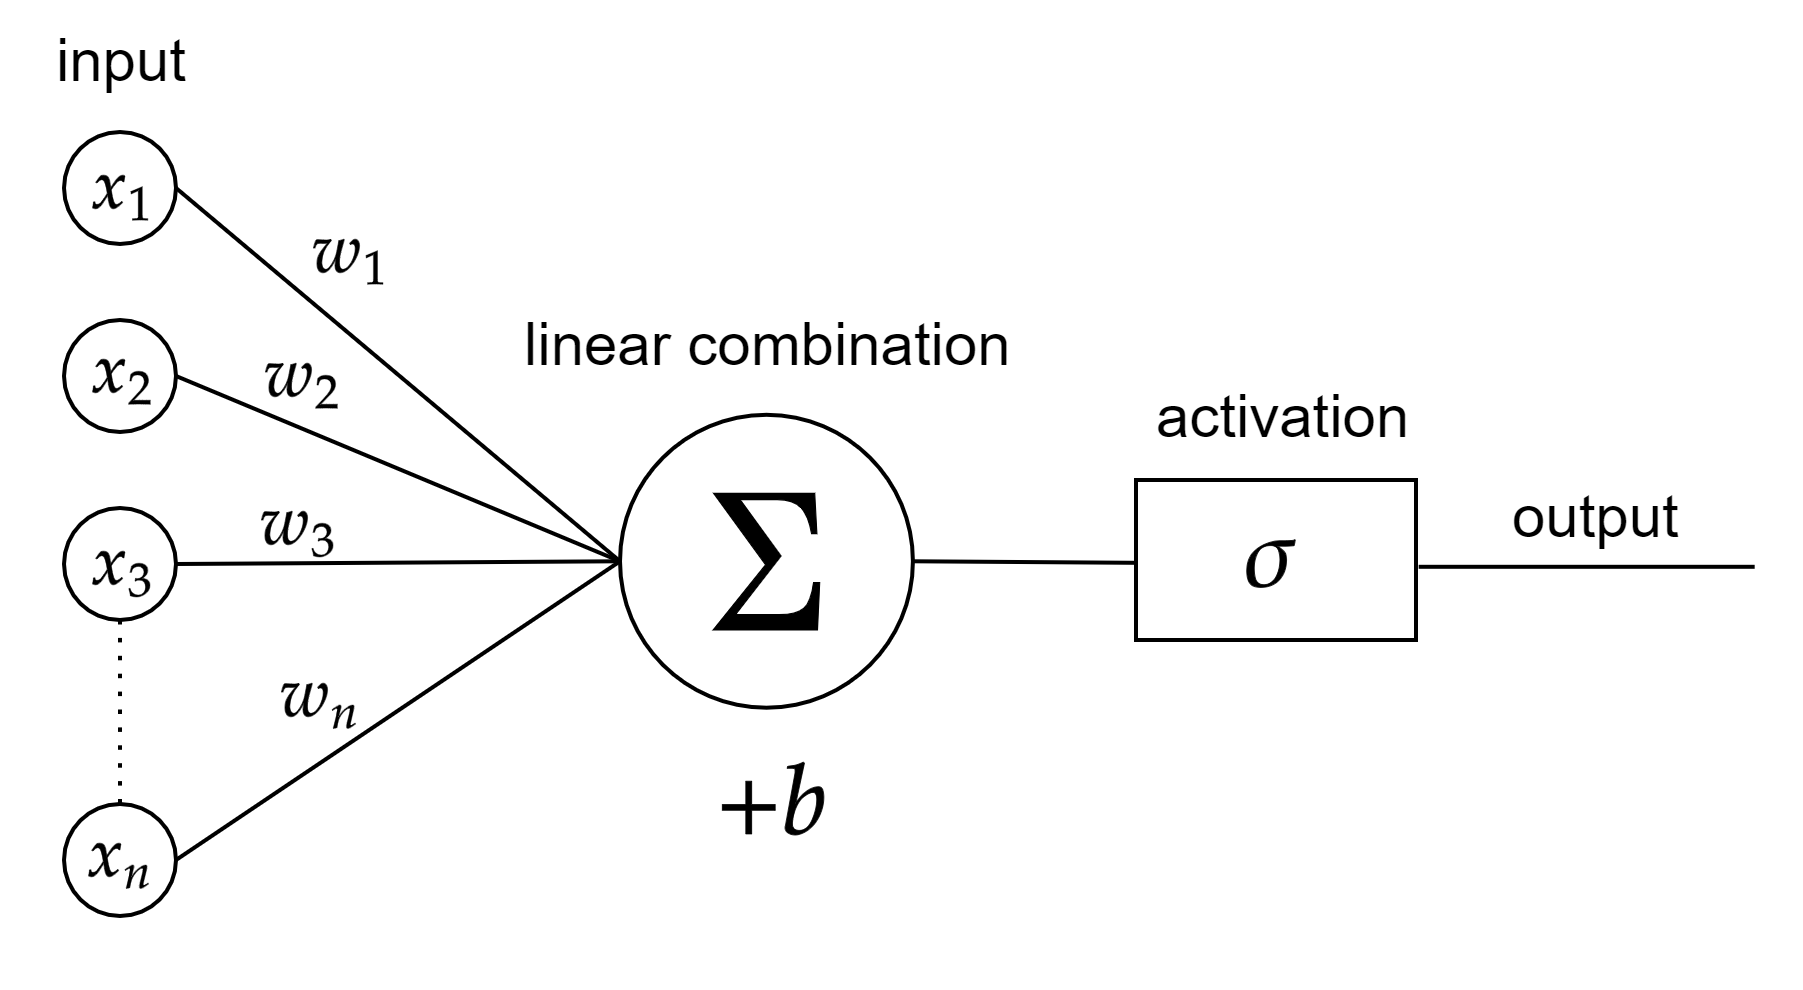
\includegraphics[scale=0.3]{img/diagram-20220205_1.png}
    \end{center}
    \caption{Illustration of the mathematical model for a single neuron.}
    \label{fig4}
\end{figure}

The choice of activation function is determined by the nature of the input and the assumed distribution of the output. When the activation function is for example equal to the Heaviside step function, as described in \cite{Rosenblatt:1958}, i.e.
\begin{equation*}
    \sigma(x) = \begin{cases} 1 & \text{if } x \geq 0, \\ 0 & \text{if } x < 0, \end{cases}
\end{equation*}
then the artificial neuron coincides with a so-called linear support vector classifier, which is a mathematical method of pattern recognition that divides a set of objects into classes in such a way that the widest possible area around the class boundaries remains free of objects, see \cite[Chapter~7]{Bishop:2006}. \\
The activation function can be any non-constant, non-linear function, but those generally used are monotone increasing, continuous, and at least piecewise smooth. At present, the most popular activation function is the rectified linear unit, abbreviated ReLu, \cref{ReLu}. In recent decades, smoother activation functions have been used, such as the sigmoid function, \cref{Sigmoid}, or the hyperbolic tangent function, \cref{TanH}, \cite[p.~3]{LeCunBengioHinton:2015}.
\begin{align}
    \sigma(y) &=\max \{y, 0\} & & \text{ rectified linear unit (ReLU) } \label{ReLu} \\
    \sigma(y) &=\frac{1}{1+\exp (-y)} & & \text{ sigmoid } \label{Sigmoid} \\
    \sigma(y) &=\tanh (y)=\frac{\exp (y)-\exp (-y)}{\exp (y)+\exp (-y)} & & \text{ hyperbolic tangent } \label{TanH}
\end{align}
Unfortunately, a single neuron is incapable of both producing a multi-dimensional output and approximating any reasonably complicated function. This led to the creation of networks of artificial neurons, known as (artificial) neural networks. Here the neurons are typically organized into multiple layers, where the input is given to several neurons simultaneously and these then compute a multidimensional output. The neurons of one layer are connected only to neurons of the immediately preceding and immediately following layers. The outputs of the neurons of one layer is utilized as inputs to the neurons of the subsequent layer. \\
We assume that we have $L \in \mathbb{N}$ layers of artificial neurons. We use $n_l$ to denote the number of neurons in layer $1 \leq l \geq L$. As input, each of the $n_l$ neurons in layer $l$ receives the output $x^{l-1} \in \mathbb{R}^{n_{l-1}}$ of the $n_{l-1}$ neurons in the previous layer $l-1$. Each neuron in layer $l$ has its own vector of weights $w_i \in \mathbb{R}^{n_{l-1}}$, $i = 1, \ldots, n_l$. The weights of all $n_l$ neurons in layer $l$ can be conveniently organized into a matrix $W \in \mathbb{R}^{n_l \times n_{l-1}}$, where the $i$-th row is the transposed weight vector $w^{\mathrm{T}}_i$ of the $i$-th neuron. We group the $n_l$ biases of the $n_l$ neurons into a vector $b \in \mathbb{R}^{n_l}$. We obtain the nl linear combinations, which is the weighted and biased input, of the nl neurons in the l-th layer via 
\begin{equation}
    \label{propagation function}
    a^l = W^l x^{l-1} + b^l \in \mathbb{R}^{n_l},
\end{equation}
which we will call propagation function of layer $l$. \\
The same activation function will be used in all neurons of layer l, which is why we define the activation function $\sigma \colon \mathbb{R} \to \mathbb{R}$ for vector-valued input values $a \in \mathbb{R}^m$ by applying it component-wise:
\begin{equation*}
    \sigma_l \colon \mathbb{R}^{n_l} \ni a^l \mapsto \sigma_l (a^l):= \left(
        \begin{array}
            {c} \sigma_l \left( a^l_{1} \right) \\
            \vdots \\
            \sigma_l \left( a^l_{n_l} \right)
        \end{array}
        \right) \in \mathbb{R}^{n_l}.
\end{equation*}
We draw attention to the fact that the activation function $\sigma_l$ can vary from layer to layer by using the index $l$. The transformation of the input $x^{l-1} \in \mathbb{R}^{n_{l-1}}$ in the $l$-th layer can then be written as
\begin{equation}
    \label{action layer}
    \mathbb{R}^{n^{l-1}} \ni \underbrace{x^{l-1}}_{\text{input of layer } l} \mapsto x^{l}:=\underbrace{\sigma_{l}\left( W^{l} x^{l-1} + b^{l} \right)}_{\text{output of layer } l}=: F_{l} \left(x^{l-1}, W^{l}, b^{l} \right) \in \mathbb{R}^{n^{l}}, 
\end{equation}
where we identify the entire process in layer $l$ with a map $F_l \colon \mathbb{R}^{n_{l-1}} \times \mathbb{R}^{n_l \times n_{l-1}} \times \mathbb{R}^{n_l} \to \mathbb{R}^{n_l}$. \\

There are many ways in which artificial neurons or layers of neurons are partitioned and connected to each other to form an artificial neural network. In this context, the term topology refers to the structure of the network, which means how many artificial neurons are located on how many layers and how they are connected to each other. However, we should focus our interest on a very specific topology of neural networks, which forms a specific class of neural networks that have proven to be of greatest practical value, namely feed-forward neural networks, abbreviated by FNN, which consist of the composition of the layer-wise action \cref{action layer}. The term feed-forward means that the information only flows in one direction, i.e. there are only connections from the neurons of one layer to the neurons of the next layer and no skipping or backward connections. Furthermore, FNNs are in general fully connected, which means that the output of each neuron in one layer would be passed to all neurons in the following layer. FNNs are also known as multilayer perceptrons, although this name can be misleading as the artificial neurons are usually not the perceptrons as introduced in \cite{Rosenblatt:1958}. \\
To simplify the notation of FNNs, we introduce a so-called input layer with $l=0$, which only receives external data and does not change the input and is the first layer of the network. The number of neurons in this layer corresponds to the dimension of the input. From now on, we will refer to the last layer of a general neural network, which produces the ultimate result, as the output layer. The number of neurons in this layer is equal to the dimension that the desired output should have. If an FNN has more than one layer, we refer to all layers between the input layer and the output layer as hidden layers. \\ 
\begin{figure}[H]
    \begin{center}
        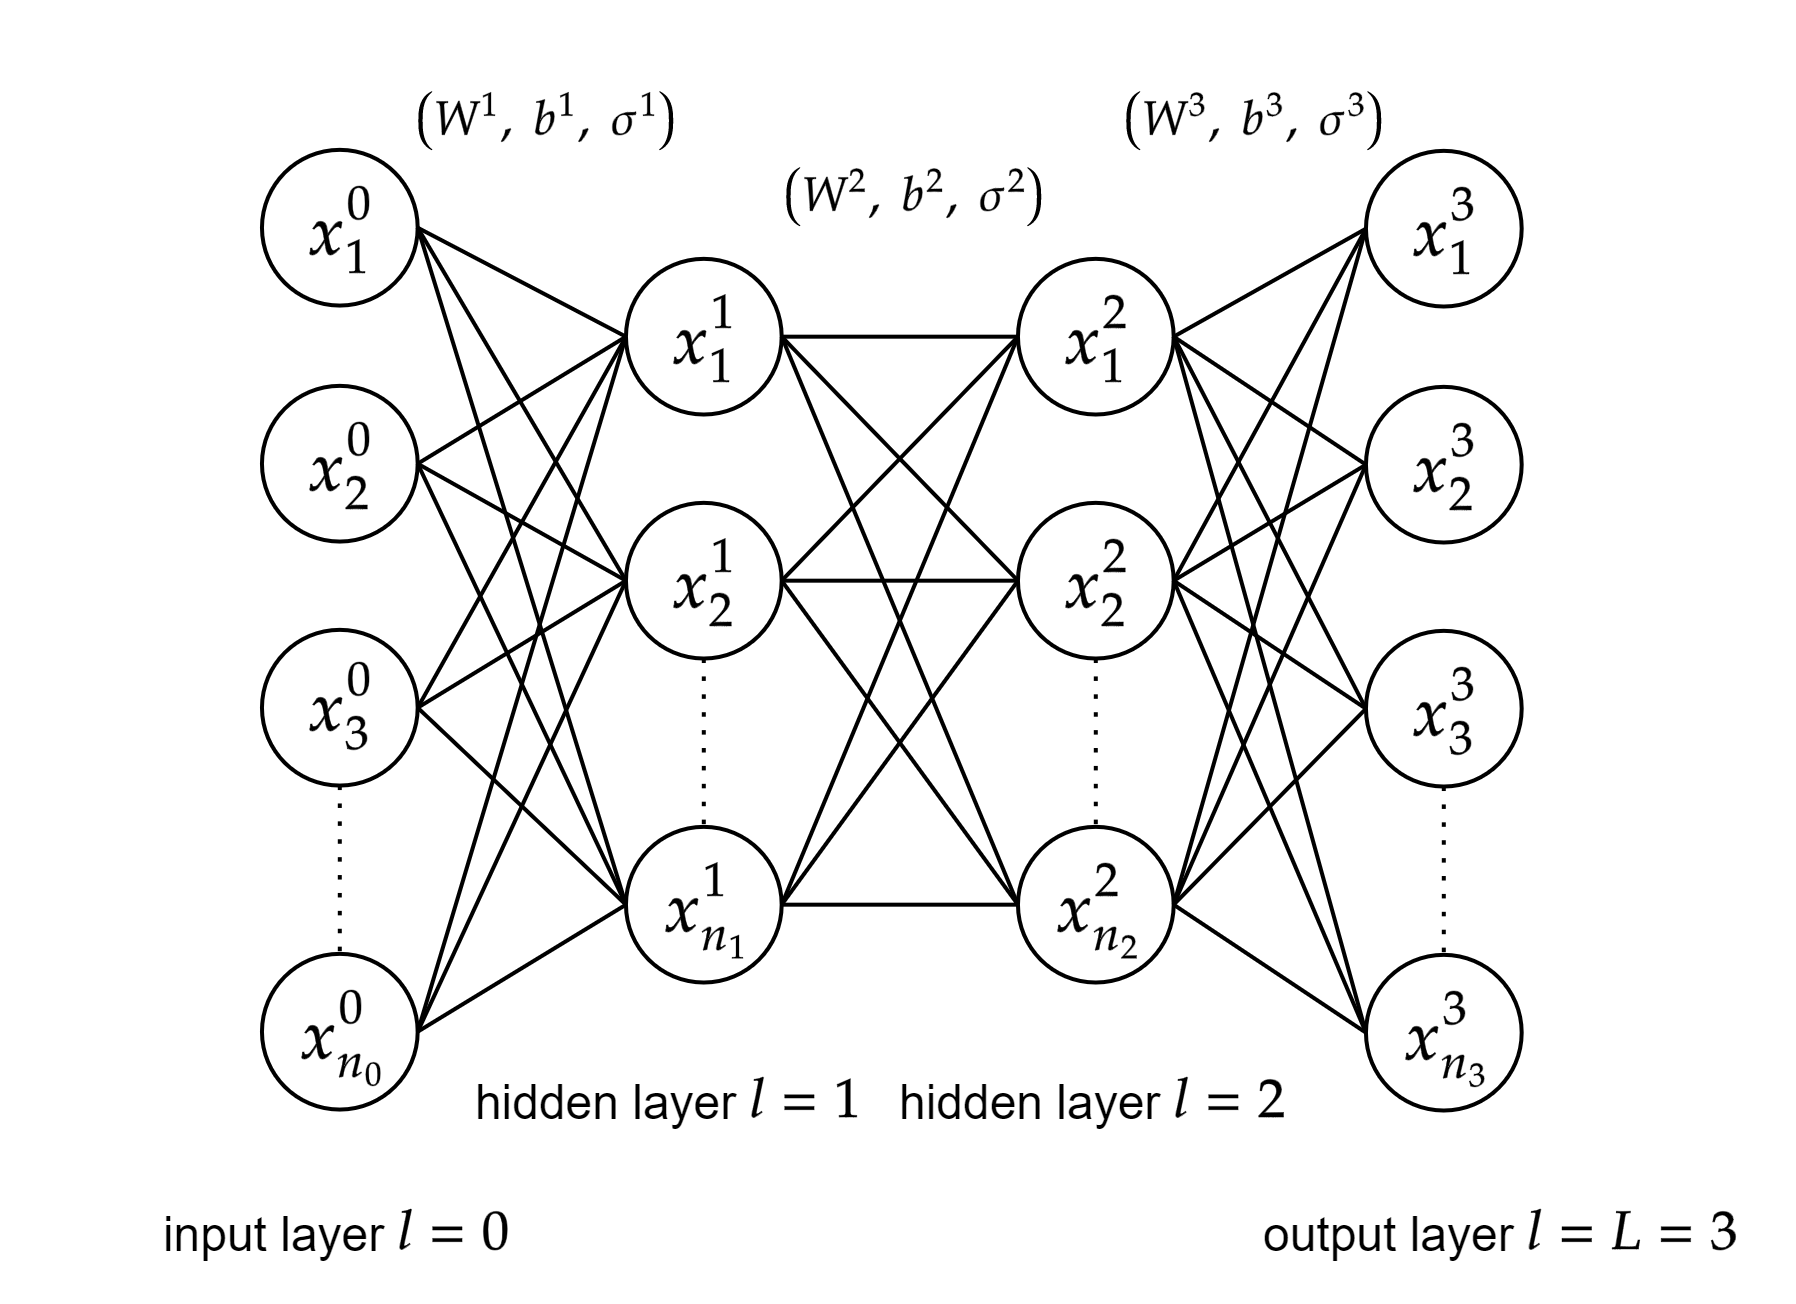
\includegraphics[scale=0.2]{img/diagram-20220206.png}
    \end{center}
    \caption{Illustration of a feed-forward neural network with $L=3$ layers.}
    \label{fig5}
\end{figure}
Neural networks can generally be represented as graphs, where the neurons are represented as vertices and the connections of the neurons are represented as edges. The input layer is sometimes also represented as a layer of vertices. An example of an FNN is illustrated in \cref{fig5}, where the network has $L=3$ layers and therefore $2$ hidden layers. The mapping of the input $x = x^0 \in \mathbb{R}^{n_0}$ to the output $y = x^3 \in \mathbb{R}^{n_3}$ by the network is given by 
\begin{equation}
    \label{forward propagation of information}
    \begin{aligned}
        y &=\sigma_{3} \left( W^{3} \sigma_{2} \left(  W^{2} \sigma_{1} \left( W^{1} x^{0}+b^{1}\right)+b^{2}\right)+b^{3}\right) \\
        &=F_{3}\left(F_{2}\left(F_{1}\left(x^{0}, W^{1}, b^{1}\right), W^{2}, b^{2}\right), W^{3}, b^{3}\right) \\
        &= F \left( x^{0}, W^{1}, b^{1}, W^{2}, b^{2}, W^{3}, b^{3} \right) \\
        & = F(x^{0}, W, b).
    \end{aligned}
\end{equation}
The process \cref{forward propagation of information} is in general called model prediction of the corresponding neural network and can be interpreted as a forward propagation of information through the neural network. From now on, we will abbreviate the model prediction of a neural network with $F(x, W, b)$, where $x = x^0$ is the input, $W = \{ W^l \}_{l = 1, \ldots, L}$ is the total of all weight matrices and $b = \{ b^l \}_{l = 1, \ldots, L}$ is the total of all bias vectors used in the network. It becomes clear that the activation functions $\sigma_l$ should be non-linear. Otherwise, the output $x^3$ is a linear function of the input $x^0$ and all layers can be combined into one output layer. \\

The neural network illustrated in \cref{fig5} can now transform values from the space $\mathbb{R}^{n_0}$ to values from space $\mathbb{R}^{n_3}$. Now the question arises how this FNN learns to solve regression problems or to approximate smooth functions $f \colon \mathbb{R}^{n_0} \to \mathbb{R}^{n_3}$. The necessary procedure is appropriately called (machine) learning. From a practical point of view, learning for a neural network means that the weights and biases of the single neurons are adjusted in such a way that for the given input the desired output is produced by the network. The most common types of machine learning are supervised learning and unsupervised learning. \\
For supervised learning, it is assumed that a so-called training data set $S = \{ (x_i, y_i) \}_{i = 1, \ldots, N}$ is given, which consists of ordered pairs of inputs $x_i$ and outputs $y_i$ of the function which should be approximated, where the output $y_i$ is the actual function value of the function to be learned for the respective input value $x_i$. The learning task is to produce the desired output $y_i$ for each input $x_i$ with the corresponding neural network. For this purpose, a cost function is defined that compares the target output values $y_i$ with the outputs generated by the network $F(x_i, W, b)$. This is in general achieved by considering the mean squared error, abbreviated MSE, which tries to minimize the average squared error between the generated outputs $F(x_i, W, b)$ and the target outputs $y_i$. Then one tries to choose the weights $W = \{ W^l \}_{l = 1, \ldots, L}$ and biases $b = \{ b^l \}_{l = 1, \ldots, L}$ so that the MSE over all data pairs $\{ (x_i, y_i) \}_{i = 1, \ldots, N}$ can be kept as small as possible. This can be defined as the following optimization problem: 
\begin{equation*}
    \begin{gathered}
        \text{ Minimize } \underbrace{\frac{1}{N}}_{\text{normalization factor}} \sum_{i=1}^{N} \lVert \underbrace{F\left(x_{i}, W^{1}, b^{1}, \ldots, W^{L}, b^{L}\right)}_{\text{model prediction }} - \underbrace{y_{i}}_{\text{actual data }} \rVert^{2}_2 \\
        \\
        \text{ where }\left(W^{l}, b^{l}\right) \in \mathbb{R}^{n_l \times n_{l-1}} \times \mathbb{R}^{n_l}, \quad l=1, \ldots, L .
    \end{gathered}
\end{equation*}
Of course, loss functions other than the MSE can be used, but the MSE has become the most common because of the differentiability it provides. \\
For unsupervised learning, only input values are given as training data, i.e. $S = \{ x_i \}_{i = 1, \ldots, N}$. In this form of machine learning, the network tries to recognise structures in the given input values. For this purpose, a cost function $C$ of the input data $x_i$ and the network's output $F(x_i, W, b)$ is defined, which is dependent on the task of the function to be approximated, such as the input domain, and any a priori assumptions, such as the implicit properties or characteristics of the function to be approximated and its arguments. One also tries to minimize the mean over all cost functions applied on $x_i$ and $F(x_i, W, b)$ with respect to the weights $W = \{ W^l \}_{l = 1, \ldots, L}$ and the biases $b = \{ b^l \}_{l = 1, \ldots, L}$, which leads to the following optimization problem:
\begin{equation*}
    \begin{gathered}
        \text{ Minimize } \; \frac{1}{N} \sum_{i=1}^{N}  C \left( F \left( x_{i}, W^{1}, b^{1}, \ldots, W^{L}, b^{L}\right), x_i \right) \\
        \\
        \text{ where } \; \left(W^{l}, b^{l}\right) \in \mathbb{R}^{n_l \times n_{l-1}} \times \mathbb{R}^{n_l}, \quad l=1, \ldots, L .
    \end{gathered}
\end{equation*}


The cost function can be much more complicated. Its form depends on the application:



In unsupervised learning, input data is given along with the cost function, some function of the data x and the network's output. The cost function is dependent on the task (the model domain) and any a priori assumptions (the implicit properties of the model, its parameters and the observed variables).


The (learning) machine tries to recognise patterns in the input data that deviate from the structureless noise.[1] An artificial neural network is guided by the similarity to the input values and adapts the weights accordingly.

During the learning phase, an unsupervised network tries to mimic the data it's given and uses the error in its mimicked output to correct itself (ie. correct its weights  biases).

The hope is that through mimicry, which is an important mode of learning in people, the machine is forced to build a compact internal representation of its world and then generate imaginative content from it.





The more complex the problem to be solved with the help of the neural network is, the more layers are needed. 

We note that the type of activation function is not learned from the data, therefore it is not in the arguments of F or F in either 3 or 4. The type of activation function, like the number of layers and the number of neurons for a layer, is a so-called hyperparameter and is determined in advance by the user. 

We would like to point out that in both optimization problems the activation functions do not appear as optimization variables. This is because hyperparameters are generally not learned. 
Choosing the right hyperparameters is extremely difficult, generally they are discovered by trial and error. 


Deep-learning methods are representation-learning methods with multiple levels of representation, obtained by composing simple but non-linear modules that each transform the representation at one level (starting with the raw input) into a representation at a higher, slightly more abstract level. With the composition of enough such transformations, very complex functions can be learned.


We compute an objective function that measures the error (or distance) between the output scores and the desired pattern of scores. The machine then modifies its internal adjustable parameters to reduce  this error. These adjustable parameters, often called weights, are real numbers that can be seen as ‘knobs’ that define the input–output function of the machine. In a typical deep-learning system, there may be hundreds of millions of these adjustable weights, and hundreds of millions of labelled examples with which to train the machine. To properly adjust the weight vector, the learning algorithm computes a gradient vector that, for each weight, indicates by what amount the error would increase or decrease if the weight were increased by a tiny amount. The weight vector is then adjusted in the opposite direction to the gradient vector. 

A deep-learning architecture is a multilayer stack of simple modules, all (or most) of which are subject to learning, and many of which compute non-linear input–output mappings. Each module in the stack transforms its input to increase both the selectivity and the invariance of the representation.

The backpropagation procedure to compute the gradient of an objective function with respect to the weights of a multilayer stack of modules is nothing more than a practical application of the chain rule for derivatives. The key insight is that the derivative (or gradient) of the objective with respect to the input of a module can be computed by working backwards from the gradient with respect to the output of that module

Many applications of deep learning use feedforward neural network architectures (Fig. 1), which learn to map a fixed-size input (for example, an image) to a fixed-size output (for example, a probability for each of several categories). To go from one layer to the next, a set of units compute a weighted sum of their inputs from the previous layer and pass the result through a non-linear function. At present, the most popular non-linear function is the rectified linear unit (ReLU), which is simply the half-wave rectifier. In past decades, neural nets used smoother non-linearities, such as , but the ReLU typically learns much faster in networks with many layers, allowing training of a deep supervised network without unsupervised pre-training28. Units that are not in the input or output layer are conventionally called hidden units. The hidden layers can be seen as distorting the input in a non-linear way so that categories become linearly separable by the last layer 


Zusammenhang zu daten
Perceptron
Activation Function
One layer
Neural Network
FNN
%ResNet
Machine Learning, Training 
Supervised Learning
Unsupervised Learning
Gradient Based optimization
Backpropagation 
NAS
Honrik 